\documentclass[border=5pt]{standalone}
\usepackage{circuitikz}
\usetikzlibrary{positioning}
\usetikzlibrary{shapes,arrows,decorations.pathreplacing}
\tikzset{block/.style = {draw, fill=white, rectangle,
              minimum height=3em, minimum width=2cm},
    input/.style = {coordinate},
    output/.style = {coordinate},
    pinstyle/.style = {pin edge={to-,t,black}},
    radiation/.style={decorate,decoration={expanding waves,angle=12,segment length=4pt}}
}
%%%%%%%%%%%%%%%%%%%%%%%
\begin{document}
  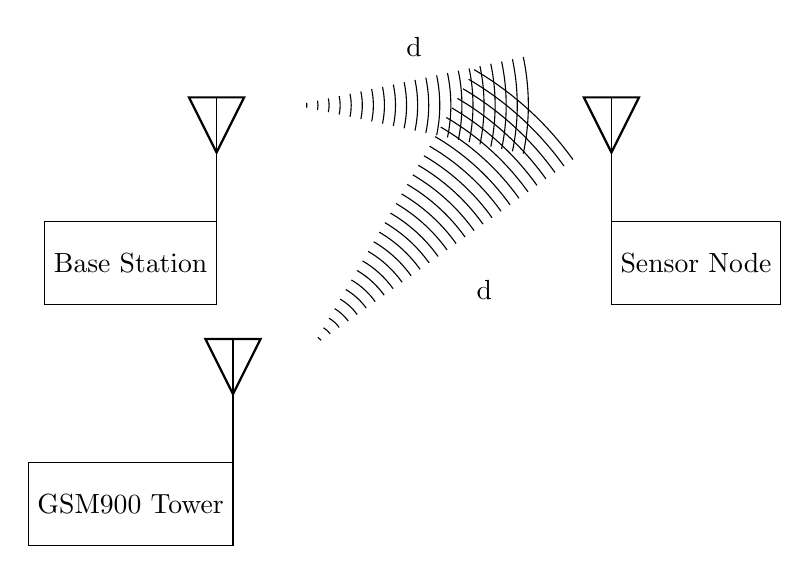
\begin{tikzpicture}[auto, node distance=2cm,>=latex']
\node[block](tx){Base Station};
\node[antenna] at (tx.east) {};
\node[block,below  = 2cm of tx](ttx){GSM900 Tower};
\node[antenna] at (ttx.east) {};
\node[block,right = 5cm of tx](rx){Sensor Node};
\node[antenna,xscale=-1] at (rx.west) {};

\draw[radiation] ([shift={(1cm,2cm)}]tx.east)-- node [above=5mm] {d} ([shift={(-1cm,2cm)}]rx.west);

\draw[radiation] ([shift={(1cm,2cm)}]ttx.east)--node [below right=8mm] {d}([shift={(-1cm,2cm)}]rx.west);
\end{tikzpicture}
\end{document} 
